\newpage
\begin{center}
\noindent\textbf{ГЛАВА 3. ВЕРХНИЕ ОЦЕНКИ ХРОМАТИЧЕСКИХ ЧИСЕЛ СФЕР}\label{chapters:3}
\vspace{1.5mm}
\end{center}

В этой главе приводятся численные результаты и некоторые теоретические рассуждения, продолжающие построения из первой главы. 
Как и раньше, будем обозначать как $G$ двойственный граф триангуляции для некоторой сферической диаграммы Вороного, 
удовлетворяющей условиям \ref{chapter1:eq:diams}, \ref{chapter1:eq:radiuseq}, $G^2$ -- его квадрат. 
Граф триангуляции для диаграмм Вороного с икосаэдральной симметрией обозначается $T(p,q)$.

\vspace{5pt}
\textbf{3.1 Численные эксперименты}\label{chapters:3.1}
\vspace{5pt}

В ходе численных экспериментов были загружены субоптимальные решения задачи Томсона, 
доступные в \textit{Cambridge Cluster Database}. 
Для них (с помощью \textit{QHull}) были построены диаграммы Вороного, двойственные графы триангуляции и их квадраты.  
Задачи о раскраске последних в $7,8,9,10$ цветов были перекодированы в задачи булевой выполнимости (в соответствии с 
формулой \ref{chapter1:eq:formula}), которые подавались на вход нескольким \textit{SAT}-решателям. 
Из полученных раскрасок квадратов двойственных графов были восстановлены раскраски сферы, вычислены диапазоны радиусов, 
при которых эти раскраски корректны (выполнены условия \ref{chapter1:eq:diams}, \ref{chapter1:eq:radiuseq}). 
Вышеперечисленные шаги были запрограммированы на ЯП Python [Приложение 2,3]. 
Наряду со стандартными функциями языка активно использовались библиотеки \textit{numpy}, \textit{scipy}, \textit{python-sat},  
библиотека для работы с графами \textit{NetworkX}.

Большая часть вычислений выполнялась на сервере с
$14$-ядерным процессором Intel\textsuperscript{\textcopyright} Xeon\textsuperscript{\textcopyright} E5-4660 v3, 
операционной системой Ubuntu. 
Основные результаты вычислений приведены на \figurename{ \ref{chapter3:fig:rad}}, где жирным выделены диапазоны радиусов, 
для которых построены корректные раскраски сферы. Более подробные данные о диапазонах радиусов приведены в Приложении 1.
Отметим, что в тех случаях, когда не удалось раскрасить квадрат двойственного графа в $8$ цветов, 
препятствием стала нехватка вычислительных ресурсов, отсутствие раскраски не было доказано.

\vspace{5pt}
\begin{figure}[h]
\centering
\begin{tikzpicture}[x=3mm,y=1em,thick,scale=1.2]
\draw (0,0) -- (25,0); %9
\draw (0,2) -- (25,2); %8
\draw (0,4) -- (25,4); %7

\draw[dashed] (0,-1) -- (0,5);
\draw[dashed] (5,-1) -- (5,5);
\draw[dashed] (10,-1) -- (10,5);
\draw[dashed] (15,-1) -- (15,5);
\draw[dashed] (20,-1) -- (20,5);
\draw[dashed] (25,-1) -- (25,5);

\draw[thickest] (3.0618621802491433,4) -- (4.33312259366566,4);
\draw[thickest] (3.8421318806398186,2) -- (4.627785868215593,2);
\draw[thickest] (4.63303264851,2) -- (6.51653329393528,2);
\draw[thickest] (10.696475079896144,2) -- (13.01019920096753,2);
\draw[thickest] (15.029181965361067,2) -- (15.376885773542428,2);
\draw[thickest] (4.538495190047897,0) -- (9.810735311262778,0);
\draw[thickest] (10.378190266191748,0) -- (10.412848135098953,0);
\draw[thickest] (10.477013319086588,0) -- (10.699936705769613,0);
\draw[thickest] (10.920307286546908,0) -- (13.359510543531439,0);
\draw[thickest] (13.427312012539147,0) -- (22.24724068159064,0);

\node[anchor=west] at (0,-1) {0};
\node[anchor=east] at (25,-1) {5};
\node[anchor=west] at (-10,2) {$\chi(S^2(r)) \leq 8$};
\node[anchor=west] at (-10,0) {$\chi(S^2(r)) \leq 9$};
\node[anchor=west] at (-10,4) {$\chi(S^2(r)) \leq 7$};
\end{tikzpicture}
\caption{Диапазоны радиусов.}
\label{chapter3:fig:rad}
\end{figure}

Отдельно рассматривался случай регулярных конфигураций $T(p,q)$: они были сгенерированы 
методом сечения икосаэдра [Приложение 4]. 
Даже при малых $p,q$ ($p,q \ge 4$) эти задачи оказываются достаточно трудоемкими: раскраска в $8$ цветов графа $T^2(5,5)$
потребовала порядка $8$ часов работы узла типа \enquote{B} вычислительного кластера \enquote{Академик В.М. Матросов}
ИДСТУ СО РАН, а также применения специализированного \textit{SAT}-решателя \textit{Cube-and-Conquer}. 
Автор и научный руководитель благодарят О.С. Заикина за помощь в решении этих задач. Полученные результаты 
сформулированы в следующем утверждении. 

\begin{statement}
\begin{equation}
\begin{split}
\chi(T^{2}(2,2)) = 8; \\
\chi(T^{2}(2,3)) = 8; \\
\chi(T^{2}(2,4)) = 8; \\
\chi(T^{2}(2,5)) = 8; \\
\end{split}
\quad\quad
\begin{split}
\chi(T^{2}(3,4)) = 8; \\
\chi(T^{2}(4,4)) = 8; \\
\chi(T^{2}(5,5)) = 8. \\
\end{split}
\end{equation}
\end{statement}

Аналогично, раскраски для больших $p,q$ не были построены ввиду ограниченности ресурсов. 
Этот результат позволяет выдвинуть следующую гипотезу.

\begin{hypothesis}
Квадраты двойственных графов регулярных (обладающих икосаэдральной симметрией) $(p,q)$-решений задачи Томсона  
являются $8$-хроматическими при $p \ge 2, q \ge 2$.
\end{hypothesis}

На разных этапах экспериментов были установлены и протестированы актуальные на момент составления текста 
версии более $10$ \textit{SAT}-решателей, среди которых
\textit{MapleSat},
\textit{Maple\-COM\-SPS-CHB},
\textit{Maple\-COM\-SPS-LRB},
\textit{Maple\-COM\-SPS-pure-CHB},
\textit{Maple\-COM\-SPS-pure-LRB},
\textit{Sat\-Elite},
\textit{Сadical},
\textit{Crypto\-Mini\-Sat5},
\textit{glu\-co\-se},
\textit{glucose-syrup},
\textit{Kissat},
\textit{Mini\-Sat},
\textit{Picosat},
\textit{lin\-ge\-ling},
\textit{plin\-ge\-ling},
\textit{treen\-ge\-ling},
\textit{RSat},
\textit{CnC}. 
Для компиляции использовался gcc 9.3.0 и опции, указанные авторами. 
В тех случаях, когда это имело смысл, замерялось время. 
На \figurename{ \ref{chapter3:fig:cactus_10}} приведены результаты замера времени работы 
(по горизонтальной оси -- количество решенных задач, по вертикальной -- суммарное затраченное время)
некоторых \textit{SAT}-решателей (с параметрами по умолчанию) для раскраски в $10$ цветов.

\begin{figure}[h]
\centering
\captionsetup{justification=centering}
\center{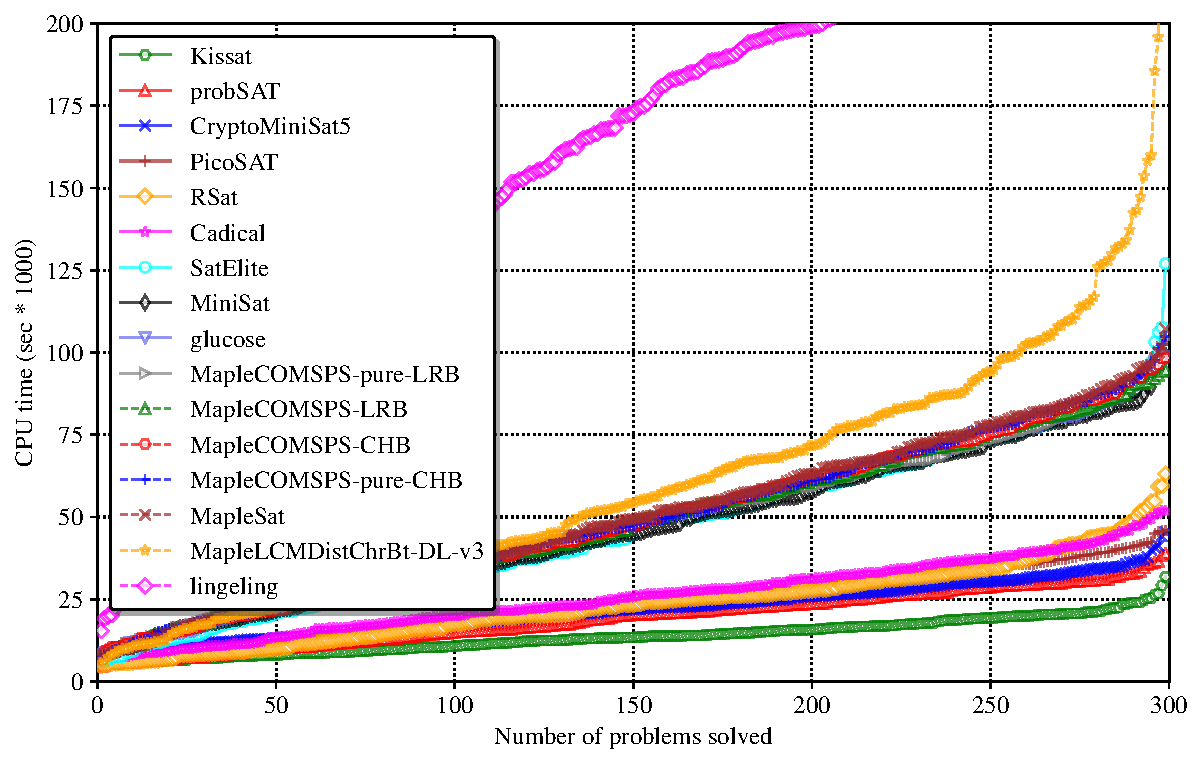
\includegraphics[width=0.7\paperwidth]{chapters/chapter3/cactus_10.pdf}}
\caption{Сравнение \textit{SAT}-решателей.}
\label{chapter3:fig:cactus_10}
\end{figure}

Анализируя эти данные автор пришел к выводу, что сравнение эффективности различных 
реализаций и комбинаций их параметров на формулах такого вида малоинформативно: 
многие из них показывают очень близкие результаты. 
Кое-что можно сказать и о самих задачах. Так, в $10$ и $9$ цветов почти мгновенно покрасились все примеры, 
конфликты встречаются редко, при росте $N$ время работы растет незначительно, что говорит о том, 
что такие задачи оказываются относительно простыми для \textit{SAT}-решателей.
С раскрасками в $8$ цветов ситуация прямо противоположная -- эта задача оказывается 
сложной для \textit{SAT}-решателей и никакие комбинации параметров не позволяют решать ее за разумное время. 
При этом удаление одной вершины степени $5$ и ее соседей снова делает ее простой. 
Представляется, что проблема возникает в момент \enquote{замыкания} раскраски в окрестности одной из таких вершин, 
решатель сталкивается с неразрешимым конфликтом и возвращается глубоко назад по дереву рекурсии.

Для визуализации построенных графов и раскрасок на языке C\texttt{++} разработана программа, 
основанная на графической библиотеке \textit{OpenGL} [Приложениe 5]. 
На \figurename{ \ref{chapter3:fig:viz}} приведены результаты работы программы для раскраски сферы в $9$ цветов, $N=192$.

\FloatBarrier
\begin{figure}[!h]
\centering
\captionsetup{justification=centering}
\begin{minipage}[b]{0.5\linewidth}
\center{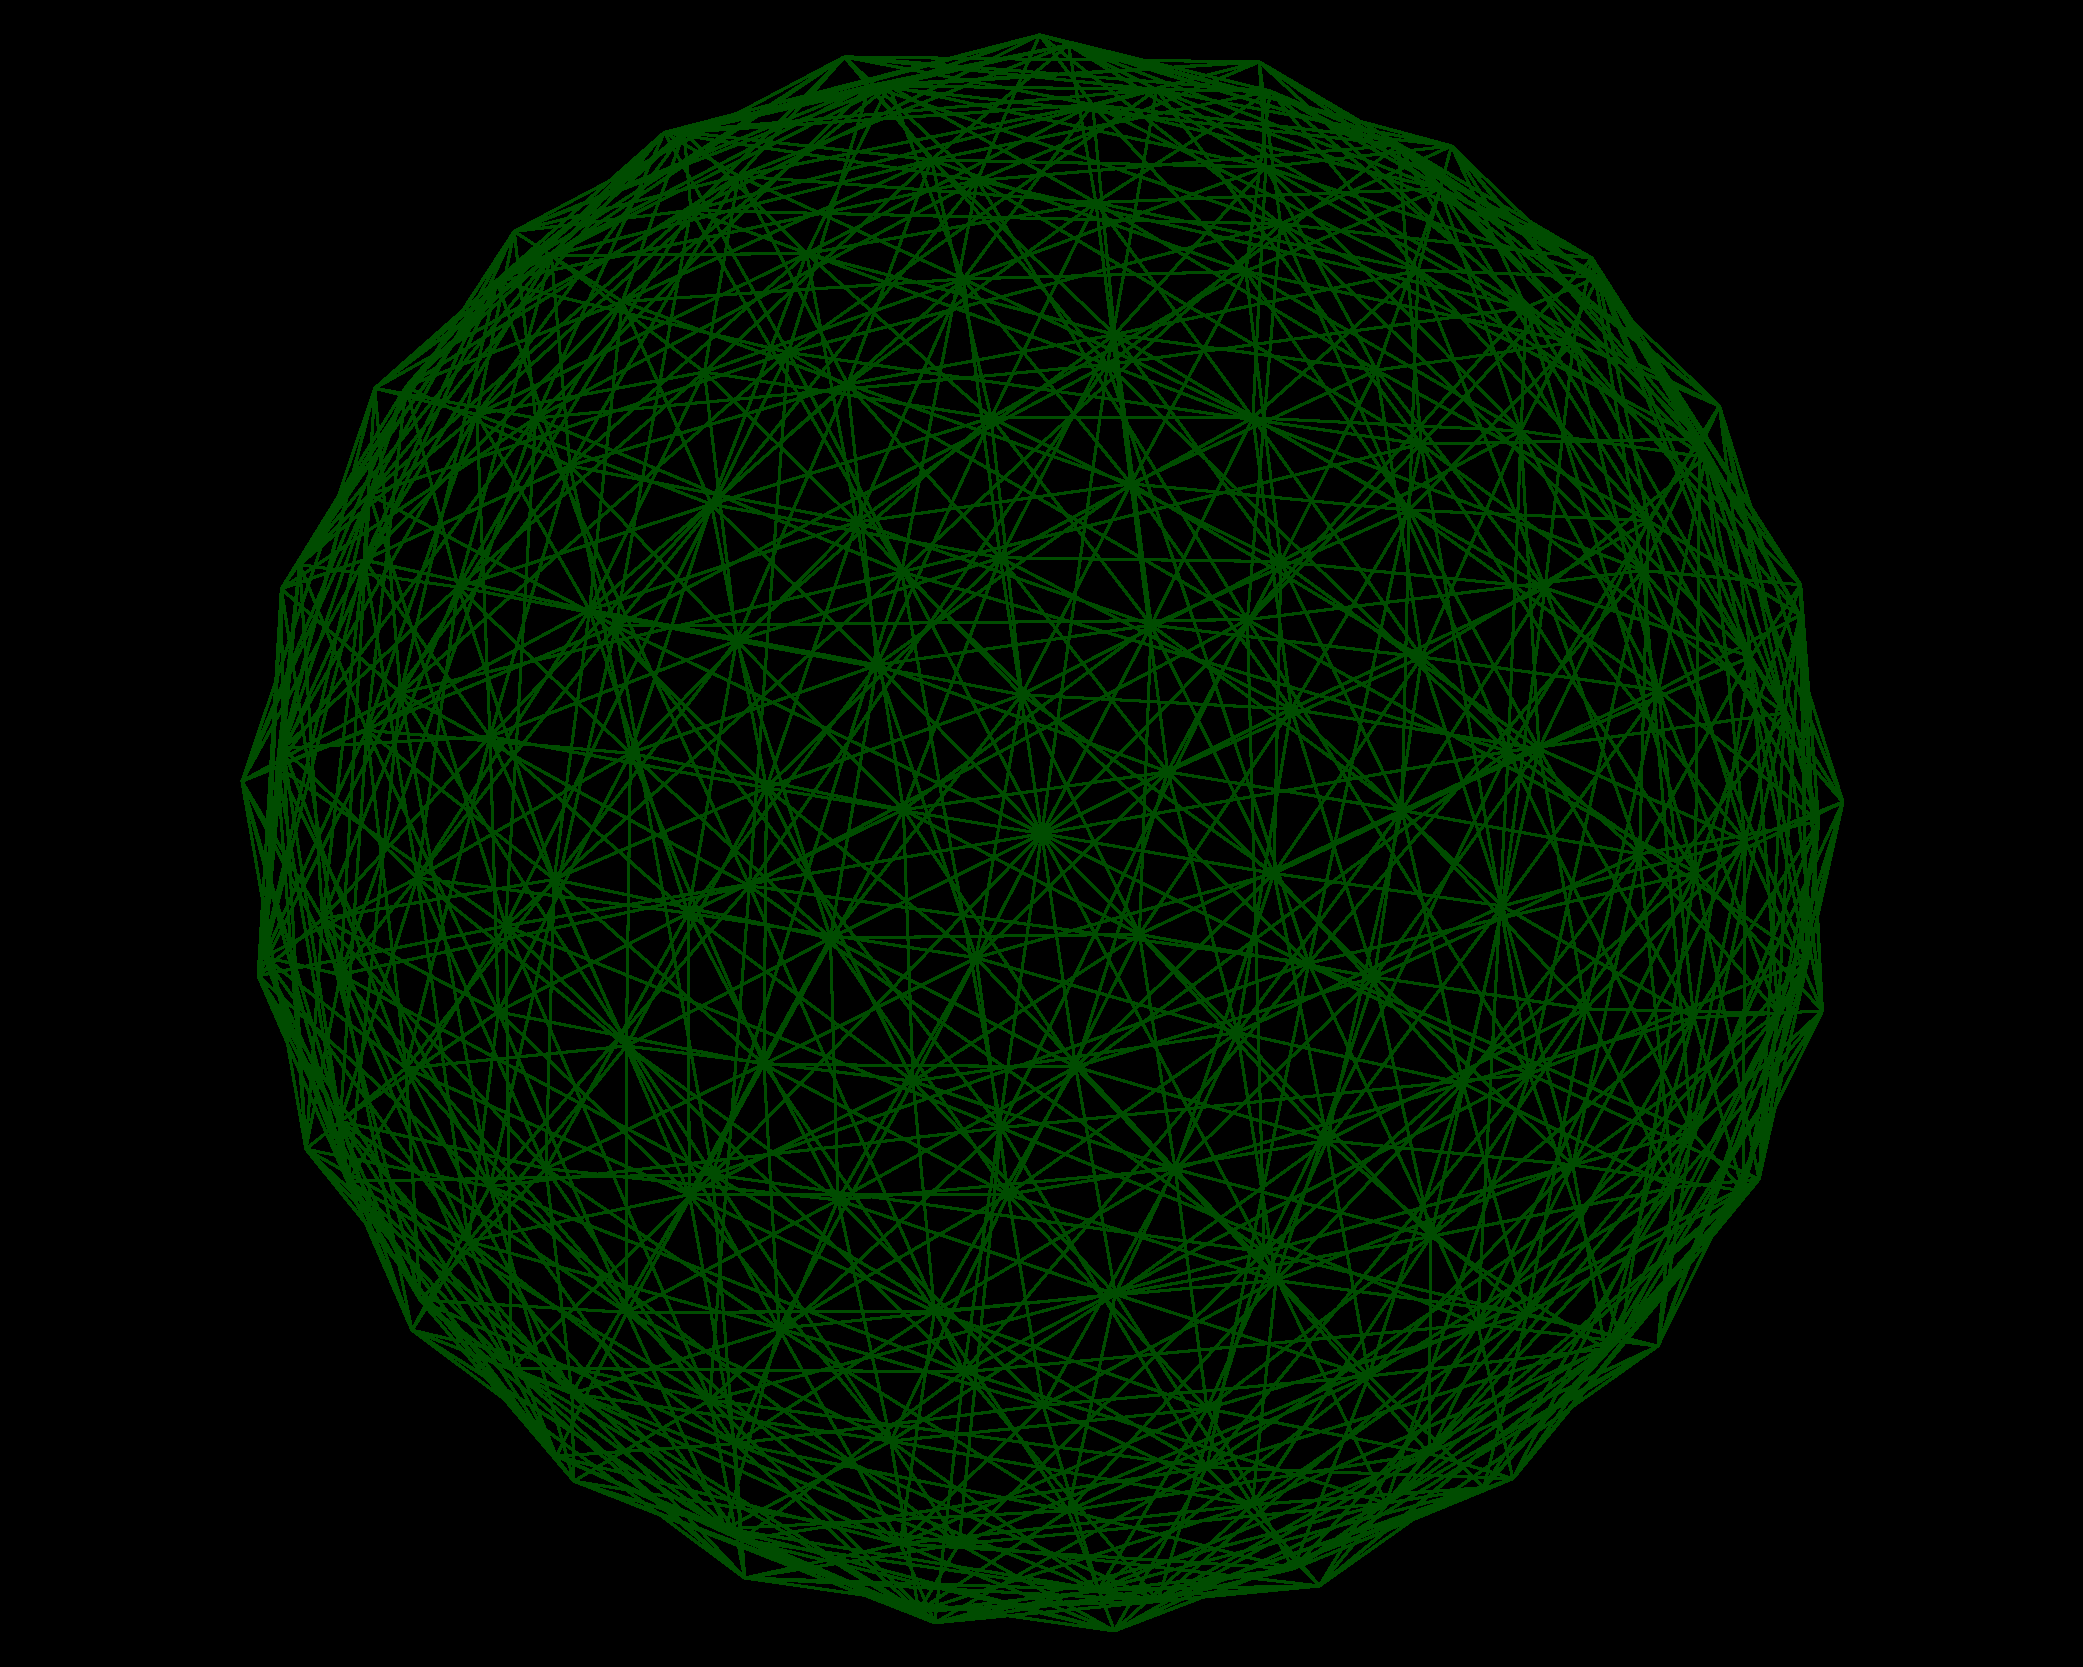
\includegraphics[width=0.37\paperwidth]{chapters/chapter3/program_viz4.pdf}}
\vspace{1ex}
\end{minipage}\hfill
\begin{minipage}[b]{0.5\linewidth}
\center{\includegraphics[width=0.37\paperwidth]{chapters/chapter3/program_viz3.pdf}}
\vspace{1ex}
\end{minipage}\hfill
\begin{minipage}[b]{0.5\linewidth}
\center{\includegraphics[width=0.37\paperwidth]{chapters/chapter3/program_viz2.pdf}}
\vspace{1ex}
\end{minipage}\hfill
\begin{minipage}[b]{0.5\linewidth}
\center{\includegraphics[width=0.37\paperwidth]{chapters/chapter3/program_viz1.pdf}}
\vspace{1ex}
\end{minipage}\hfill
\caption{Пример визуализации раскраски.}
\label{chapter3:fig:viz}
\end{figure}

\vspace{5pt}
\textbf{3.2 Теоретические оценки}\label{chapters:3.2}
\vspace{5pt}

\begin{lemma}\label{chapter3:lemma}
Пусть $G$ содержит такую вершину $v$ степени $5$, что каждая из смежных с ней вершин имеет степень $6$. 
Тогда $\chi(G^2) \ge 8$. В частности, при $p,q \ge 1$ выполнено $\chi(T^2) \ge 8$.
\end{lemma}

\begin{figure}[h]
\centering
\captionsetup{justification=centering}
\center{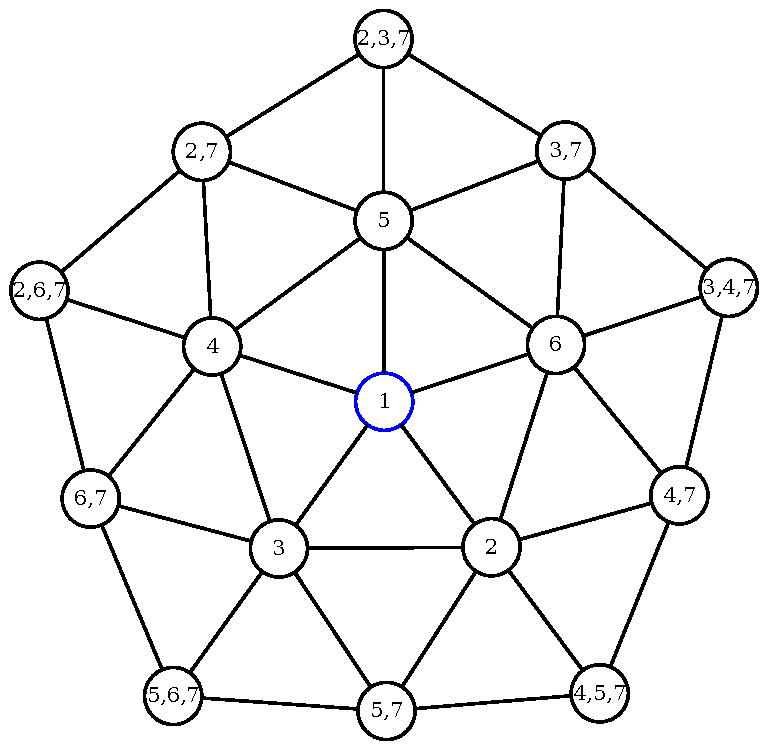
\includegraphics[width=0.45\paperwidth]{chapters/chapter3/cap.pdf}}
\caption{К лемме \ref{chapter3:lemma}.}
\label{chapter3:fig:lemma}
\end{figure}

\begin{proof}
На \figurename{ \ref{chapter3:fig:lemma}} приведены возможные цвета вершин в окрестности вершины степени $5$ (без ограничения общности). 
Тогда из вершин \enquote{внешнего} пояса не более трех имеют цвет $7$, а остальные $7$ вершин раскрашены в цвета $2$--$6$. Но это невозможно, поскольку из этих $7$ вершин можно покрасить в любой из цветов $2$--$6$ не более одной. 
\end{proof}




В заключение приведем основной теоретический результат данной работы.

\begin{theorem}\label{chapter3:theorem}
При $r \geq r_0 = \sqrt{\frac{153^2}{1220}}$ для раскраски областей сферической диаграммы Вороного,
удовлетворяющей условиям \ref{chapter1:eq:diams}, \ref{chapter1:eq:radiuseq}, 
потребуется по крайней мере $8$ цветов.
\end{theorem}

\begin{myproof}
Пусть $T$ -- двойственная триангуляция диаграммы Вороного. 
Предположим, что существует правильная раскраска $T^2$ в $7$ цветов.
Тогда $T$ не содержит вершины  степени $7$ или более (для раскраски ее $1$-окрестности потребуется $8$ цветов).
Поскольку суммарный дефект вершин равен $12$, число вершин в ненулевым дефектом не больше $12$. 
Назовем такие вершины \textit{дефектными}.

Заметим, что раскраска полоски ширины $4$, состоящей из шестиугольников, определяется однозначно конечным участком 
(на \figurename{ \ref{chapter3:fig:hex_determ}} последовательно раскрашиваются шестиугольники $a,\,b,\,c,\,d$). 
Это рассуждение, разумеется, можно сформулировать и в терминах раскрасок $T$.

\begin{figure}[h]
\centering
\captionsetup{justification=centering}
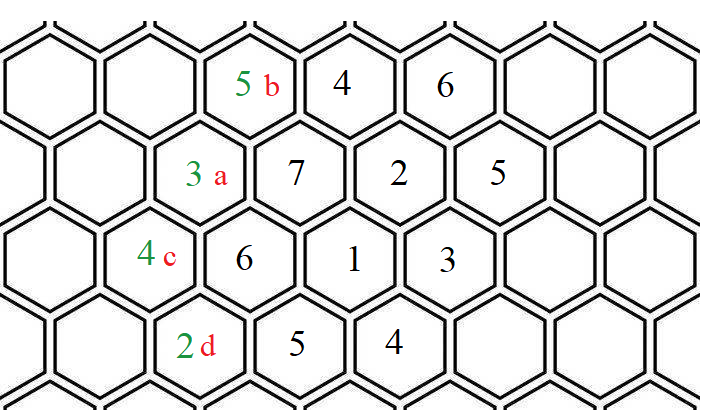
\includegraphics[width=10cm]{chapters/chapter3/hex_determ.png}
\caption{К теореме \ref{chapter3:theorem}.}
\label{chapter3:fig:hex_determ}
\end{figure}

Пусть $T_1$ -- подграф $T$, полученный как объединение всех $4$-окрест\-нос\-тей дефектных вершин; 
$T_2$ -- подграф $T_1$, состоящий из вершин $T_1$, находящихся на расстоянии не более $4$ от некоторой вершины из 
$V(T) \backslash V(T_1)$. Предположим, что $T_2$ непуст. Очевидно, $T_2$ является планарным, как и $T$. 
Любой цикл на этом графе разбивает графы $T, \, T_2$ на две части в смысле укладки на плоскости (сфере) и теоремы Жордана. Обозначим внутреннюю часть $\operatorname{int} L$.

\begin{lemma}
Пусть правильная раскраска $T$ в 7 цветов существует, и $L=(v_1,v_2, \dots , v_l, v_1)$ -- некоторый простой цикл на $T_2$. 
Тогда сумма дефектов вершин $T$ внутри (снаружи) $L$ делится на 6.
\end{lemma}

\begin{myproof}

Рассмотрим допустимую раскраску $T$ (и вершин $L$) в 7 цветов. 
Припишем каждой упорядоченной паре цветов $(i,j)$ направление 
$\phi_{ij}=k\pi/3$, $k \in \{ \, 0, 1, \dots , 5 \, \}$, соответствующее переходу между данной парой в раскраске плоскости. 
Каждой паре соседних вершин $v_s, v_{s+1}$ соответствует некоторое направление $\phi_s$, 
причем при обходе $L$ оно остается неизменным, если эта вершина имеет $2$-x соседей внутри и $2$-x вне $L$, 
иными словами, если к ней внутри и вне $L$ примыкает по $3$ треугольника триангуляции, порожденной вложением $T$ в плоскость. 
Если снаружи $4$ треугольника, а внутри -- $2$, то  $\phi_{s+1}=\phi_s-\pi/3$ и т.~д.:
$$\phi_{s+1}-\phi_{s} = \frac{\pi}{6} \left( \Delta_{in}(v)- \Delta_{out}(v) \right),$$
где $\Delta_{in}(v)$, $\Delta_{out}(v)$ -- число треугольников, примыкающих к вершине, 
соответственно, внутри и снаружи области, ограниченной путем $L$. 

Назовем дефектом пути число

$$\delta(L) = \sum\limits_{s} \frac{1}{2} \left(\Delta_{in}(v_s) - \Delta_{out}(v_s) \right).$$
Для любого замкнутого пути на триангуляции из формулы Эйлера следует, что 

$$\delta(L) = 6 - \sum\limits_{v \, \in \, \operatorname{int} L} \delta(v).$$
Остается заметить, что $$\sum\limits_{s=1}^l \left(\phi(v_{s+1}) - \phi(v_s)\right) = 2\pi k = \frac{\pi}{3} \delta(L),$$ 

$$\delta(L)=6k.$$

\end{myproof}

Продолжая доказательство основной теоремы, рассмотрим два случая.

1. Граф $T_2$ пустой. Тогда каждая $4$-окрестность дефектной вершины содержит не более $1+5+10+15+20=51$ вершины, 
а общее число вершин не превосходит $12 \cdot \frac{51}{2} = 306$. 
Площадь области диаметра $1$ на сфере радиуса $r$ оценивается сферху площадью сферического сегмента
$$S_i \leq S_{max} = 2 \pi r^2 \left(1- \sqrt{1-\frac{1}{4r^2}}\right).$$
Запишем неравенство для площади сферы:

$$ 612 \pi r^2 \left(1- \sqrt{1-\frac{1}{4r^2}}\right) \geq 4 \pi r^2; $$

$$ 1- \sqrt{1-\frac{1}{4r^2}} \geq \frac{1}{153}; $$

$$ \sqrt{1-\frac{1}{4r^2}} \leq \frac{152}{153}; $$

$$ 1-\frac{1}{4r^2} \leq \frac{152^2}{153^2}; $$

$$ \frac{1}{4r^2} \geq 1 - \frac{152^2}{153^2} = \frac{305}{153^2}; $$

$$ 4r^2 \leq \frac{153^2}{305}; $$

$$ r \leq \sqrt{\frac{153^2}{1220}} \approx 4.38. $$

2. Граф $T_2$ непуст. Тогда число вершин в $T$, вообще говоря, не ограничено комбинаторными соображениями, 
но дефектные вершины должны образовывать два подмножества с общим дефектом $6$ в каждом, 
а длина пояса из шестиугольников между этими двумя группами вершин не превосходит $20$, 
и этот пояс покрывает \enquote{экватор} сферы. Следовательно,

$$ 20 r \cdot 2 \arcsin \frac{1}{2 r} \geq 2 \pi r; $$

$$ \arcsin \frac{1}{2 r} \geq \frac{\pi}{20}; $$

$$ \frac{1}{2 r} \geq \sin \frac{\pi}{20}; $$

$$ r < \frac{1}{2 \sin \frac{\pi}{20}} \approx \frac{10}{\pi} \approx 3.18. $$

\end{myproof}